\documentclass[a4paper]{article}
\usepackage{amsfonts}
\usepackage{amsmath}
\usepackage{amssymb}
\usepackage{graphicx}     

\begin{document}
  
\noindent \large Auteur: Victoria Mazur \\
\noindent \large Studierichting: Informatica\\
\noindent \large Oefeningenreeks 5F nr. 3.7\\

\medskip

\normalsize

$I = \dfrac{1}{2}\displaystyle\int_{0}^{\pi}(1+\cos\theta)^{2}d\theta - \dfrac{1}{2}\displaystyle\int_{0}^{\tfrac{\pi}{2}}(\cos\theta)^{2}d\theta$ \\

$= \dfrac{1}{2}\displaystyle\int_{0}^{\pi}\left(1+2\cos\theta+\cos^{2}\theta\right)d\theta - \dfrac{1}{2}\displaystyle\int_{0}^{\tfrac{\pi}{2}}\cos^{2}\theta d\theta$ \\

$= \dfrac{1}{2}\left[\theta\right]_{0}^{\pi} + \left[\sin\theta\right]_{0}^{\pi} + \dfrac{1}{2}\displaystyle\int_{0}^{\pi}\cos^{2}\theta d\theta - \dfrac{1}{2}\displaystyle\int_{0}^{\tfrac{\pi}{2}}\cos^{2}\theta d\theta$ \\

$= \dfrac{\pi}{2} + 0 + \dfrac{1}{2}\displaystyle\int_{0}^{\pi}\cos^{2}\theta d\theta - \dfrac{1}{2}\displaystyle\int_{0}^{\tfrac{\pi}{2}}\cos^{2}\theta d\theta$ \\

$= \dfrac{\pi}{2} + \dfrac{1}{2}\displaystyle\int_{0}^{\pi}\left(\dfrac{\cos 2\theta +1}{2}\right)d\theta - \dfrac{1}{2}\displaystyle\int_{0}^{\tfrac{\pi}{2}}\left(\dfrac{\cos 2\theta +1}{2}\right)d\theta$ \\

$= \dfrac{\pi}{2} + \dfrac{1}{4}\displaystyle\int_{\tfrac{\pi}{2}}^{\pi}(\cos 2\theta +1)d\theta$ \\

$= \dfrac{\pi}{2} + \dfrac{1}{4}\displaystyle\int_{\tfrac{\pi}{2}}^{\pi}\cos 2\theta d\theta + \dfrac{1}{4}\displaystyle\int_{\tfrac{\pi}{2}}^{\pi}1d\theta$ \\

$= \dfrac{\pi}{2} + \dfrac{1}{8}\left[\sin 2\theta\right]_{\tfrac{\pi}{2}}^{\pi} + \dfrac{\pi}{8}$ \\

$= \dfrac{\pi}{2} + \dfrac{\pi}{8} = \dfrac{5\pi}{8}$ \\

\begin{figure}[h]
\centering
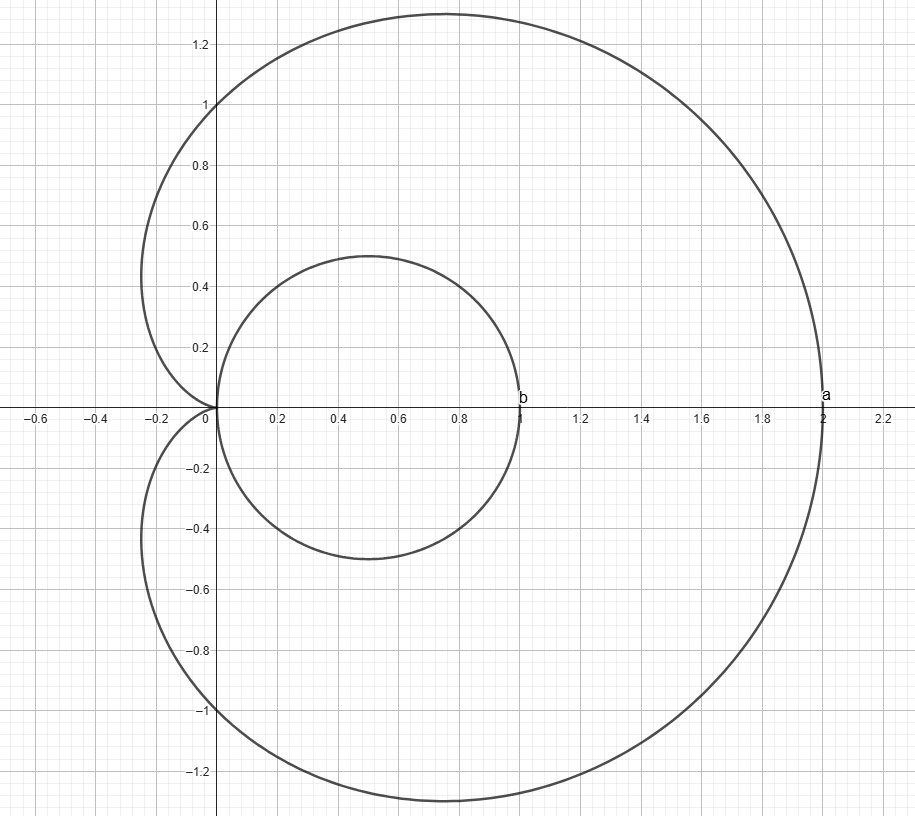
\includegraphics[width=10cm]{5F-3.7-victoria.mazur.INF.png}
\end{figure}

\begin{thebibliography}{999}
%\bibitem{a} Referentie
\end{thebibliography}
\end{document}